\begin{center}
\fbox{\fbox{\parbox{6.5in}{\centering
\begin{flushleft}

\vspace{2mm}
\hspace{5mm}
\textbf{\underline{Püramiidi elemendid}}

\vspace{2mm}
\hspace{5mm}
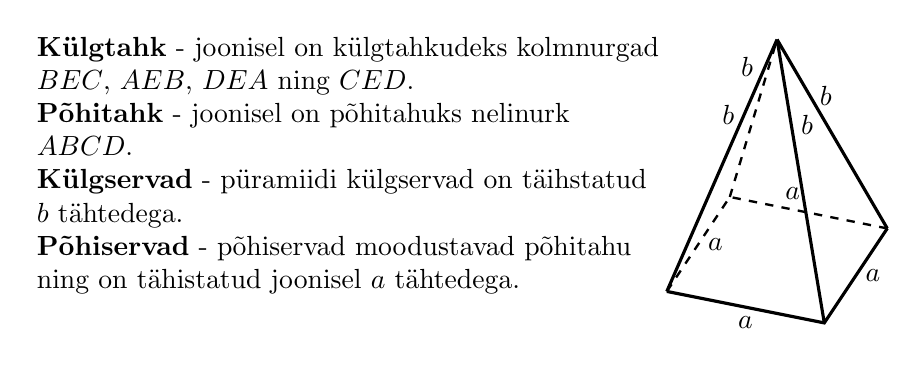
\begin{tikzpicture}[scale=0.4]
\coordinate (A) at (0,0);
\coordinate (B) at (5,-1);
\coordinate (D) at (2,3);
\coordinate (C) at (7,2);
\coordinate (E) at (3.5,8);

\draw[line width= 0.4mm] (A)--(B)--(C) (A)--(E) (B)--(E)  (C)--(E) ;
\draw[line width=0.3mm, dashed] (D)--(E) (C)--(D)--(A);

\path (A)--(B) coordinate[pos=0.5](a1);
\path (B)--(C) coordinate[pos=0.5](a2);
\path (C)--(D) coordinate[pos=0.6](a3);
\path (D)--(A) coordinate[pos=0.5](a4);

\node[below] at (a1) {$a$};
\node[right] at (a2) {$a$};
\node[above] at (a3) {$a$};
\node[right] at (a4) {$a$};

\path (A)--(E) coordinate[pos=0.7](b1);
\path (B)--(E) coordinate[pos=0.7](b2);
\path (C)--(E) coordinate[pos=0.7](b3);
\path (D)--(E) coordinate[pos=0.7](b4);

\node[left] at (b1){$b$};
\node[right] at (b2){$b$};
\node[right] at (b3){$b$};
\node[above left] at (b4){$b$};

\node[text width=8cm] at (-10,4){\textbf{Külgtahk} - joonisel on külgtahkudeks kolmnurgad $BEC$, $AEB$, $DEA$ ning $CED$.\\
\textbf{Põhitahk} - joonisel on põhitahuks nelinurk $ABCD$.\\
\textbf{Külgservad} - püramiidi külgservad on täihstatud $b$ tähtedega.\\
\textbf{Põhiservad} - põhiservad moodustavad põhitahu ning on tähistatud joonisel $a$ tähtedega.};
\end{tikzpicture}
\hspace{5mm}
\begin{tikzpicture}[scale=0.4]
\coordinate (A) at (0,0);
\coordinate (B) at (5,-1);
\coordinate (D) at (2,3);
\coordinate (C) at (7,2);
\coordinate (E) at (3.5,8);

\draw[line width= 0.4mm] (A)--(B)--(C) (A)--(E) (B)--(E)  (C)--(E) ;
\draw[line width=0.3mm, dashed] (D)--(E) (C)--(D)--(A);
\node[left] at (A){$A$};
\node[right] at (B){$B$};
\node[right] at (C){$C$};
\node[left=2mm] at (D){$D$};
\node[above] at (E){$E$};

\path (B)--(C) coordinate[pos=0.5](a2);
\path (a2)--(E) coordinate[pos=0.3](m);
\node[blue, right] at (m){$m$};
\draw[blue, line width= 0.3mm] (a2)--(E);
\pic [draw, angle radius = 3mm , line width=0.3mm] {angle=E--a2--B} node at (5.7,0.5){$\cdot$};

\coordinate (H) at (3.5,1);
\pic [draw, angle radius = 4mm , line width=0.3mm] {angle=C--H--E} node at (3.8,1.4){$\cdot$};

\draw[line width=0.3mm, dashed, red] (E)--(H);

\path (H)--(E) coordinate[pos=0.4](H1);
\node[left, red] at (H1){$H$};

\draw[line width=0.3mm, dashed] (A)--(C) (B)--(D);
\end{tikzpicture}

\vspace{2mm}
\hspace{5mm}
Püramiidi \textbf{kõrgus} on alati risti põhitahuga ning on tähistatud joonisel tähega $H$. Püramiidi kõrgus\\ \hspace{5mm} määrab põhitahu ja püramiidi tipu vahelist kaugust.\\ \hspace{5mm}
 Püramiid on \textbf{korrapärane}, kui tema põhjaks on korrapärane hulknurk ja kõik külgservad on võrdsed.\\ \hspace{5mm} 
\textbf{Apoteem} - korrapärase püramiidi tipust tõmmatud külgtahu kõrgus (joonisel tähistatud tähega $m$).

\vspace{2mm}
\hspace{5mm}
\textbf{\underline{Korrapärase püramiidi pindala}}

\vspace{2mm}
\hspace{5mm}
Kui uurida püramiidi ehitust, siis on näha, et kogu püramiidi pindala võrdub kõikide külgtahkude\\ \hspace{5mm} pindalade ja põhitahu pindala summaga. Ehk:

\begin{equation}
\label{42_eq1}
S_{t}=S_{p}+S_{k1}+S_{k2}+...+S_{kn}
\end{equation}

\hspace{5mm}
kus $S_{t}$ on püramiidi täispindala, $S_{p}$ püramiidi põhja pindala, $S_{k1}$, $S_{k2}$ jne on püramiidi külgtahkude\\ \hspace{5mm} pindalad.

\vspace{2mm}
\hspace{5mm}
Lühemalt näeks see valem välja nõnda:

\begin{equation}
\label{42_eq2}
\boxed{S_{t}=S_{p}+S_{k}}
\end{equation}

\hspace{5mm}
kus $S_{p}$ on endiselt põhja pindala ning $S_{k}$ on kõikide külgtahkude pindalade summa, ehk:\\ \hspace{5mm} $S_{k}=S_{k1}+S_{k2}+S_{k3}+...+S_{kn}$

\vspace{2mm}
\hspace{5mm}
Tasub rõhutada, et kuna püramiidil on külgtahkudeks kolmnurgad, siis võiksid kolmnurga lahendamise\\ \hspace{5mm} võtted meil käepärast olla (kasulikuks võivad osutuda peatükkid \ref{40_peatükk} ja \ref{ruut} kolmnurga osa). Põhja pindala\\ \hspace{5mm} aga sõltub kujundist.

\vspace{2mm}
\hspace{5mm}
\textbf{\underline{Püramiidi ruumala}}

\vspace{2mm}
\hspace{5mm}
Püramiidi ruumala on võrdne ühe kolmandikuga põhja pindala ja kõrguse korrutisest. Ehk:

\begin{equation}
\label{42_eq3}
\boxed{V=\dfrac{S_{p}H}{3}}
\end{equation}

\hspace{5mm}
kus $V$ on püramiidi ruumala, $S_{p}$ püramiidi põhja pindala ning $H$ on püramiidi kõrgus.
\end{flushleft}
}}}
\end{center}

\pagebreak
\vspace{0.5cm}

\textbf{Märkmed}\\
\vspace{2mm}
\begin{mdframed}[style=graphpaper]
\vspace{20cm}
\end{mdframed}